\documentclass{wptemp}
\usepackage{adjustbox}
\usepackage{dcolumn}    % aligning decimals
    \newcolumntype{d}[1]{D{.}{.}{#1}}
% *****************************************************************
% Estout LaTeX wrapper
% *****************************************************************

%%Original code developed by Jörg Weber: see
%% https://www.jwe.cc/2012/03/stata-latex-tables-estout/
%% and
%% https://www.jwe.cc/blog/


\let\estinput=\input % define a new input command so that we can still flatten the document

\newcommand{\estwide}[3]{
		\vspace{.75ex}{
			%\textsymbols% Note the added command here
			\begin{tabular*}
			{\textwidth}{@{\hskip\tabcolsep\extracolsep\fill}l*{#2}{#3}}
			\toprule
			\estinput{#1}
			\bottomrule
			\addlinespace[.75ex]
			\end{tabular*}
			}
		}	

\newcommand{\estauto}[3]{
		\vspace{.75ex}{
			%\textsymbols% Note the added command here
			\begin{tabular}{l*{#2}{#3}}
			\toprule
			\estinput{#1}
			\bottomrule
			\addlinespace[.75ex]
			\end{tabular}
			}
		}

% Allow line breaks with \\ in specialcells
\newcommand{\specialcell}[2][c]{%
    \begin{tabular}[#1]{@{}c@{}}#2\end{tabular}
}

\newcommand{\sym}[1]{\rlap{#1}}% Thanks David Carlisle


%%%%%%%%%%% End of wrapper %%%%%%%%%%%%%%%%%%%%%
    
%%%%%%%%%%% TiKz %%%%%%%%%%%%%%%%%%%%%
\usepackage{tikz}
\usetikzlibrary{shapes.geometric, arrows}

\tikzstyle{startstop} = [rectangle, rounded corners, minimum width=3cm, minimum height=1cm,text centered, draw=black, fill=red!30]

\tikzstyle{io} = [trapezium, trapezium left angle=70, trapezium right angle=110, minimum width=3cm, minimum height=1cm, text centered, text width =5cm, draw=black, fill=blue!30]

\tikzstyle{process} = [rectangle, minimum width=3cm, minimum height=1cm, text centered, text width =5cm, draw=black, fill=orange!30]

\tikzstyle{decision} = [diamond, minimum width=3cm, minimum height=1cm, text centered, draw=black, fill=green!30]

\tikzstyle{arrow} = [thick,->,>=stealth]

\begin{document}

\linespread{1}{\title{{\fontfamily{ptm}
\selectfont{\Large{\MakeUppercase{The Impact of Hispanic Last Names and Identity on Labor Market Outcomes}}}}}}
	\author{{\fontfamily{pbk}\selectfont\large{\textsc{Hussain Hadah}}\thanks{Department of Economics, University of Houston, 206A McElhinney Hall, 3623 Cullen Boulevard, Houston, TX 77204-5019, United States (e-mail: \email{hhadah@uh.edu}).}}}
	\date{\fontfamily{pbk}\selectfont\normalsize{\textsc{\today}}}
	\maketitle

\begin{center}
\href{https://hhadah.github.io/hispanic-last-names/my_paper/Hadah-last-names.pdf}{\textcolor{green!15!black!30!blue}{\footnotesize{\textsc{Click Here to Get the Most Updated Version}}}}
\end{center}
	
\pagenumbering{arabic}

\begin{abstract}
In this paper, I compare the children of inter-ethnic marriages to study the impact of having a Hispanic last name. While men born to Hispanic father-White mothers earn less than those born to White father-Hispanic mothers, the gap could be explained entirely by educational differences. I also study the effect of identifying as Hispanic on earnings. I find that men that identify as Hispanic earn significantly less than those that do not, even after controlling for educational differences. 
\end{abstract}

\pagebreak

%\section{Questions}
%
%In this paper, I will answer the following questions:
%
%\begin{enumerate}
%\item Do Hispanics face discrimination in the labor market due to an ethnic signal (last name)?
%
%\item Does the marriage market penalize or reward Hispanics for their ethnicity? 
%
%\item How do Hispanic men and women fare in inter-ethnic marriages? 
%
%\item Is there assortative matching in inter-ethnic marriages?
%
%\item Is there a difference in identity cost for those that identify as Hispanics and those that I induce are Hispanic through their parents' place of birth?
%
%\item What are the minority groups that faced a marriage market penalty? (Historical analysis)
%
%\item How did the marriage market penalty change over time for the different minority groups?
%
%\end{enumerate}
\section{Introduction}\label{sec:intro}

There is a plethora of evidence of ethnic and racial discrimination in the labor market \citep{bayer2018divergent, charles2008prejudice, card1992school, fryer2004causes, rubinstein2014pride, bertrand2004emily, juhn1991accounting}. Hispanics constitute a large and growing portion of the population in the United States. As the number of Hispanics keeps increasing in the labor force, determining whether ethnic discrimination affects their labor market outcomes becomes increasingly crucial \citep{chettyUnitedStatesStill2014, chettyEffectsExposureBetter2016,chettyFadingAmericanDream2017,abramitzkyImmigrantsAssimilateMore2020a, abramitzkyNationImmigrantsAssimilation2014,abramitzkyCulturalAssimilationAge2016,chettyWhereLandOpportunity2014}, how identity could shift public opinions toward trade \citep{grossmanIdentityPoliticsTrade2021}, and how racial and gender attitudes affect the racial and gender earnings gaps \citep{charlesPrejudiceWagesEmpirical2008,charlesEffectsSexismAmerican2018}. Thus, it is important to understand whether a person's ethnicity affects their labor market outcomes. Assimilation and mobility are crucial because they reflect how well Hispanics can integrate into society and move up the socioeconomic ladder.

In this paper, I answer the following questions. Does having a Hispanic last name affect labor market outcomes? What is the effect of identifying as Hispanic on earnings? Moreover, I aim to show that comparing Hispanic Whites to non-Hispanic Whites might create an artificially higher earnings gap since the two groups differ on many observable characteristics.\footnote{By identifying as Hispanic, I refer to individuals who self-report their ethnicity as Hispanic on surveys or other data collection instruments.} \footnote{Observable characteristics refer to factors that can be measured and quantified, such as education level, work experience, and immigration status.} Others have attempted to compare how native-born White Hispanics fare to non-Hispanic Whites and foreign-born Hispanics. In \citet{antman2020ethnic,antmanEthnicAttritionObserved2016,antmanEthnicAttritionObserved2016a,antmanEthnicAttritionAssimilation2020}, the authors compare the health and educational outcomes of Hispanic Whites to non-Hispanic Whites and native-born Hispanics to foreign-born Hispanics. They find gaps in education and health between Hispanics and Whites. They also find that native-born Hispanics are more likely than their foreign-born counterparts to report poor health. \citet{davilaChangesRelativeEarnings2008}, the authors documents many gaps in labor market outcomes between Hispanics and Whites. They attribute a big part of this gap to differences in education, experience, immigration status, and regional differences. 

The US population is growing in diversity. The proportion of non-Whites has increased by more than 10 percentage points from 1995 to 2019 (see figure \ref{fig:1}), and the number of Hispanics has grown by 9 percentage points over the same period (see figure \ref{fig:2}). Native-born White Hispanic men earn 21\% less than White men \citep{duncan2018identifying}. However, a substantial portion of the earnings gap is due to educational differences between Hispanics and Whites \citep{duncan2006hispanics, duncan2018socioeconomic}. Therefore, understanding discrimination against Hispanics and their children is an important task. Discrimination against Hispanics has a couple of negative consequences, for example discrimination against Hispanics can lead to reduced job opportunities, lower wages, and hindered assimilation. First, if Hispanics face a substantial labor market penalty for their ethnic identity, it could hinder assimilation and integration. Second, a significant labor market penalty contributes to the growing wage gap between Whites and other minority groups. In this paper, I examine the role of having a Hispanic last name and identifying as Hispanic on labor market outcomes. 

Identifying discrimination is difficult because of factors that affect labor market outcomes that are unobservable to economists---like innate ability. Also, I should be able to disentangle skills differentials between Hispanics and non-Hispanic Whites.\footnote{Skills differentials refer to differences in education, work experience, and other factors that can affect a person's job performance and wages.} To causally identify ethnic discrimination against Hispanics and its effects on labor market outcomes, a researcher should compare two identical people that only differ in their last name. Since this approach is unfeasible, researchers took different approaches. \citet{bertrand2004emily} and \citet{fryer2004causes} conducted audit studies to examine the effect of Black sounding names on employment discrimination. This approach, however, has its drawbacks. Audit studies only observe callbacks, not wages. 

This study utilizes a method developed by \citet{rubinstein2014pride} in this research. I will compare children from inter-ethnic marriages. More precisely, I will reach children of Hispanic fathers and White mothers (henceforth HW) to children of White fathers and Hispanic mothers (henceforth  WH). This approach stems from the fact that marriages are not random. Couples match on several observable characteristics like income, schooling, socio-economic background, etc. \citep{averettBetterWorseRelationship2008, averettEconomicRealityBeauty1996, beckerTheoryMarriagePart1973, beckerTheoryMarriagePart1974, beckerTreatiseFamily1993, browningCollectiveUnitaryModels2006, chiapporiFatterAttractionAnthropometric2012}. Children of HW and WH marriages have more similar observable characteristics than children of homogeneous marriages--- i.e., White fathers-White mothers and Hispanic fathers-Hispanic mothers. Moreover, children from a Hispanic father and White mother household will have a Hispanic last name from their fathers, enabling the investigation of how ethnic signals, such as having a Hispanic last name, affect annual log earnings.

Using the Current Population Survey (CPS) from 1994 to 2019 and the 1970-1990 US censuses, I will estimate the effect of having a Hispanic last name on the labor market outcomes. In other words, I will approximate the variation in labor market perception of ethnic signals, in this case having a Hispanic last name, on annual log earnings. I also study the effect of identifying as Hispanic on labor market outcomes. 

To retrieve the effect of having a Hispanic last name, I compare the children of inter-ethnic marriages between Whites and Hispanics. I find that while men born to White father-Hispanic mothers earn less than men born to Hispanic father-White mothers, this gap is entirely explained by educational differences. Thus, I do not find a significant effect of having a Hispanic last name. Finally, I find that men identifying as Hispanic earn significantly less than those who do not, even when I control ancestry and education. Inter-ethnic children with a White father, and thus having a non-Hispanic last name, earn 14\% less than children of endogamous White parents. Inter-ethnic children with a Hispanic father, and thus having a Hispanic last name, earn 20\% less than children of endogamous White parents. Endogamous children with Hispanic parents earn 24\% less than children of endogamous White parents. A big part of the gaps could be explained by education. Inter-ethnic children with a White father and identify as Hispanic, and thus having a non-Hispanic last name, earn 14\% less than children of endogamous White parents. Inter-ethnic children with a Hispanic father and identify as Hispanic, and thus having a Hispanic last name, earn 18\% less than children of endogamous White parents. Endogamous children with Hispanic parents and identify as Hispanic earn 10\% less than children of endogamous White parents.

A long list of economic papers investigated taste-based discrimination, statistical discrimination, and Black-White and gender earnings gaps that date back to the seminal work of \citet{becker2010economics}. \citet{bayer2018divergent} investigated the Black-White wage gap's narrowing and then divergence. \citet{card1992school} argued that the Black-White wage gap narrowed from 1960 to 1980 due to improvement in the quality of Black schools, and \citet{juhn1991accounting} showed that skills play a big part in the Black-White wage gap. Moreover,  \citet{charles2008prejudice} provided evidence that 25\% of the Black-White wage gap is due to prejudice. \citet{black1995discrimination} introduced a search model showing that with a taste for discrimination, minorities earn less than the majority group even when hired by an unprejudiced firm. In comparison, \citet{altonji2001employer} found that firms do not statistically discriminate based on race and ethnicity. Little has been done, however, about discrimination against Hispanics, which offers an opportunity to exploit the observable racial similarities between Hispanics and Whites.

Previous studies have also used names as a proxy for race and ethnicity \citep{fryer2004causes, rubinstein2014pride, bertrand2004emily}. \citet{fryer2004causes} point out that names can be a predictor of a person's race. Specifically, they provide a rising pattern among Blacks having different names than Whites. They did, however, find that having a Black name, after controlling for the home environment at birth, does not affect their labor market outcomes. \citet{rubinstein2014pride} compared the children of mixed marriages between Sephardic and Ashkenazis in Israel.\footnote{Ashkenazi and Sephardic are two distinct Jewish ethnic groups.} They found that workers with Sephardic last names earn substantially less than those with an Ashkenazi last name. \citet{bertrand2004emily} conducted an audit study by sending employers identical resumes that differ in the ethnic and racial signal of a name (Black sounding name versus a White sounding one). They found that resumes with Black-sounding names received substantially fewer callbacks than their White counterparts. 

The rest of the paper is organized as follows. Section \ref{sec:data} provides an overview of the data and summary statistics of the sample I am using. Section \ref{sec:emp_model} introduces a formal empirical model. I go over the results in section \ref{sec:results}. Finally, I offer a brief conclusion in section \ref{sec:con}.

\section{Data}\label{sec:data}

For this paper, I will use two data sets. The Integrated Public Use Microdata Series (IPUMS) Current Population Survey (CPS) Annual Social and Economic (ASEC) \citep{cps2019} and the 1970 to 1990 US censuses \citep{acs2019}. 

I use the CPS' rich data set to study the effect of having a Hispanic last name on a person's labor market outcomes. I take advantage of the fact that the CPS asks for parents' place of birth, ethnicity, and race. The data spans the period between 1994--- the earliest sample to ask about a parent's place of birth--- to 2019. Moreover, since the CPS does not provide data on parents' characteristics, essential to determine the family background, I use the census to construct synthetic parents. The census offers a larger sample of potential parents. Similar to the CPS, the 1970 to 1990 censuses ask about the person's place of birth and the individual's race and ethnicity. I employ this information to construct "synthetic parents" using a method developed by \citet{rubinstein2014pride}. I construct the synthetic parents by linking husbands and wives in the census data to each other. I assume that parents have children between the ages of 25 and 40, I then link these synthetic parents using the year they were surveyed to the year of birth of the "children" in the CPS sample.

\subsection{Children of the four parental types}
I will use the CPS for my primary analysis of the effect of having a Hispanic last name on earnings. I restrict my sample to Whites, United States-born citizens aged 25 to 40 and born between 1970 to 1990. Taking advantage of data on parents' place of birth, I divide the sample into four groups depending on their parent's ethnicity. Mothers or fathers are Hispanic if they were born in a Spanish-speaking country and Puerto Rico, and White if they were born in the United States.\footnote{The list of Spanish Speaking countries include: Argentina, Bolivia, Chile, Colombia, Costa Rica, Cuba, Dominican Republic, Ecuador, El Salvador, Guatemala, Equatorial Guinea, Honduras, Mexico, Nicaragua, Panama, Paraguay, Peru, Spain, Uruguay, Venezuela.} Therefore, an observation can be the product of four types of parents: 
\begin{enumerate}
\item White father and White mother (hereafter WW) 
\item White father and Hispanic mother (hereafter WH)
\item Hispanic father and White mother (hereafter HW)
\item Hispanic father and Hispanic mother (hereafter HH).
\end{enumerate}
The distribution of the four types of children is presented in figure \ref{fig:dist}. The majority of the sample, 95.14\%, is WW children. The second biggest group is HH, which constitutes 3.36\% of the sample. Inter-ethnic children, WH and HW, make up 1.78\% of the sample with 60,147 observations. Even though WH and HW are only 1.78\% of the sample, I have plenty of observations to carry out an analysis. The summary statistics for the children of the four types of marriages are presented in table \ref{tab:c&p1}. Children of WW marriages (column i) do better on every measure while children of HH parents (column iv) do worse than other children on every measure. 


On the one hand, WW children are more educated, with approximately 14 years of education for men and women. man and woman WW children have an employment rate of 95\%. They have log hourly earnings of 2.557 for men and 2.435 for women. Also, their annual log earnings are 10.529 for men and 10.297 for women.

On the other hand, children of HH marriages have an average of 12.898 and 13.204 years of education for men and women, respectively. HH men and women have an employment rate of 93\%. Their annual log earnings are 10.365 and 10.175 for men and women, respectively. 

Inter-ethnic children, WH and HW, have lower educational attainment and income than WW children, but they are better than HH children. Also, WH and HW are comparable, unlike WW and HH children. These two groups are important to the analysis. Children of HW are going to be the treatment group. HW's children have a Hispanic father, who will carry his Hispanic last name. At the same time, the WH children have White fathers and will take his non-Hispanic, or White, last name. A first glance at the summary statistics of these two groups, table \ref{tab:c&p1} columns (ii) and (iii) can show that they are different from the children of non-inter-ethnic marriages. 

WH children have an average of 13.366 and 13.741 years of education for men and women. The employment rate for men is 94.5\% and for women 95.0\%. HW man and woman children obtained 13.072 and 13.270 years of schooling. Men's employment rate is 92.7\% and women's 93.1\%.

In panel D of table \ref{tab:c&p1}, I present the rates at which members of each group self-identify as Hispanic \footnote{Hispanic self-identification is observed when an individual notes that they are Hispanic on the CPS questionnaire}. The vast majority of HH children, 97\%, identify as Hispanic. There is considerable attrition in Hispanic identification of inter-ethnic children. Among WH children, 82.1\% of men and 85.0\% of women identified as Hispanic. Among HW children, 87.9\% of men and 85.9\% of women identified as Hispanic. These results align with the findings of a substantial body of literature that noted this attrition among children of immigrants, especially those coming from inter-ethnic marriages \citep{duncan2017complexity, duncan2018identifying, duncan2020new, antman2020ethnic}. Finally, a small portion of WW children, 6\%, identified as Hispanic. These 6\% of WW children are most likely third generation--- or more--- immigrants. For my analysis, I dropped the WW observations identified as Hispanic to compare with non-Hispanic Whites.

In columns (v) and (vi), I calculate the differences in means between HH-WW (column v) and HW-WH (column vi). Overall, HH children do worse than WW children. HH has one less year of education compared to WW, 2.1 percentage points less likely to be employed, HH men earn 18\% less than WW men, and HH women make 12.3\% less than WW women. Therefore, these two groups, HH and WW, are different in many observable.

The differentials between WH and HW are not as severe as the ones between HH and WW. HW children are still worse off than WH but are way better than HH. HW men attain 0.294 fewer years of education than WH men. HW women achieve 0.471 fewer years of schooling than WH women. HW children are 1.8-1.9 percentage points less likely to be employed. HW men earn the same annual earnings as WH men, and HW women earn 10.3\% less. These differences show that HW and WH children are different from children of homogeneous marriages and, thus, are more comparable.

Moreover, in table \ref{tab:c&p2}, I present the summary statistics for the four types and limit the sample to those that only identify as Hispanic\footnote{Limiting the sample to those that identify as Hispanic only affects WH, HW, and HH. Members of the WW group are not affected by this restriction.}. The same pattern discussed above between HH--WW and HW--WH persists. The one difference is that those who identify as Hispanic do slightly worse.

 %In columns five and six of table \ref{tab:c1}, I present the gaps between HH and WW children and HW and WH children, respectively. The gap between HH and WW children (column five) shows a consistent story, HH children are worse in education and work more. HH children have more kids. While the gap between HW and WH does not have a clear-cut direction. Even though WH children obtain more years of education and have a higher employment rate, HW and WH men have the same fertility rates. HW women have a higher fertility rate than WH women. WH and HW women have the same employment rate.
 
\subsection{Synthetic parents}

Using the 1970 and 1990 censuses, I constructed a panel of synthetic parents. The sample includes married White men and women. Even though the census asks a person whether they are Hispanic or not, I took advantage of the questions on place of birth to create a proxy for ethnicity. I consider a Hispanic person as White and born in a Spanish-speaking country. Consequently, Whites in the sample are people who are White and native-born. Using the information provided in the census, I can link husbands and wives with each other. I assume that parents have children between the ages of 25 and 45. Therefore, my sample consists of married White men and women that were born in the 1930 to 1965 cohorts\footnote{The construction of "synthetic parents" follows the method used by \citet{rubinstein2014pride}.}.

I show the distribution of the four types of couples in table \ref{tab:mat1}. White husbands and White wives (WW) make up the majority of couples in the sample, 98.18\% (681,206 couples). Hispanic husbands and wives (HH) are the second largest group making up 1.04\% (7,193 couples)of all couples. White husbands and Hispanic wives (WH) couples are 0.40\% (2,750 couples) of the sample while Hispanic husbands and White wives (HW) are 0.39\% (2,710 couples). 


I present the summary statistics of the four types of synthetic parents in table \ref{tab:c&p1}'s parent's panel. WW couples have higher education, 11.9 years for husbands and 11.8 for wives. As a household, WW couples have 25.194 years of schooling. Husbands in HH marriages have 8.5 years of education, while women have 8.2 years of schooling. As a household, HH couples have 17.539 years of education.

WH husbands have 10.3 years of education, while wives have an average of 9.6 years, the lowest of any group. WH household attained a total of 22.308 years of schooling in total. HW husbands and wives obtained 9.7 and 9.8 years of education, respectively. HW household attained a total of 21.473 years of schooling in total.

In columns (v) and (vi) of table \ref{tab:c&p1}, I calculated the differences in means between HH-WW households and HW-WH households. An HH Hispanic husband attained 3.779 fewer years of education than a WW husband. While an HH wife acquired 3.876 fewer years of schooling than a White WW wife. The total educational difference between HH and WW households equals 7.655 years of education. The educational differences between HW and WH are less severe than those between HH and WW. A Hispanic husband in intermarriage attained 1.560 fewer years of schooling than a White husband in intermarriage. A White wife in intermarriage attained 0.726 years of education, more than a Hispanic wife in intermarriage. The difference in total years of education between HW and WH households is 0.835, which is an 89\% decrease from the HH--WW gap. These differences show that couples that intermarry are better and different than those that do not.

%In table \ref{tab:p1} columns five and six, I provide the  HH-WW and HW-WH gaps. WW couples are more educated and earn more than HH couples. Also, WH husbands are more educated and earn more than HW husbands. In comparison, WH wives are more educated than HW wives. Even though White husbands in intermarriages are more educated and earn more than husbands in HW marriages, they are more comparable to each other than the non-intermarriage couples.

\section{Empirical Strategy}\label{sec:emp_model}
In this section, I will present two empirical strategies. The first empirical strategy will estimate the effect of having a Hispanic last name on annual log earnings. The second empirical strategy will estimate the effect of identifying as Hispanic on log yearly earnings.

The difference in means between Hispanics and non-Hispanic Whites could result from discrimination. It can also be caused by differences in innate abilities, skills, and parental investments during infancy. To avoid these threats to identification, I compare children of inter-ethnic marriages, HW and WH. WH and HW children are equally Hispanic physically but provide employers/labor market with different signals.\footnote{WH and HW children are both half White, half Hispanic.} WH children will have a non-Hispanic last name, while HW children will have a Hispanic last name. This is a method developed by \citet{rubinstein2014pride}.

\section{Estimating the effect of having a Hispanic last name}

Let $Y_{ist}$ be the annual log earnings of person $i$ in state $s$ at time $t$. $WH_{ist}$, $HW_{ist}$ and $HH_{ist}$ are indicator variables for the type of parents person $i$ has. $X_{ist}$ is a vector of controls, $\gamma_{t}$ are year fixed effects, $\lambda_{s}$ are state fixed effects, and $\phi_{ist}$ represents the error term. The equation for this strategy is written as follows:
\begin{equation} \label{eq:1a}
Y_{ist} = \beta_{1} WH_{ist} +\beta_{2} HW_{ist} + \beta_{3} HH_{ist} + X_{ist} \pi + \gamma_{t} + \lambda_s + \phi_{ist}
\end{equation}

$\beta_{1}, \beta_{2}$ and $\beta_{3}$ are the coefficients of interest in this specification. They estimate the earnings gaps between the three groups and children of White-White parents. The difference between $\beta_{1}$ and $\beta_{2}$ captures the effect of having a Hispanic last name. This comes from the fact that the WH and HW children are similar. On the one hand, WH children will have a White father and carry his White last name. On the other hand, HW children will have a Hispanic father and carry his Hispanic last name. Therefore, \textit{ceteris paribus}, the difference will capture the effect of having a Hispanic last name.

\subsection{Estimating the effect of identifying as Hispanic}

In this section, I will present an estimation strategy that would allow me to capture the effect of identifying as a Hispanic. The empiricism in the section follows the theoretical identity model developed by \citet{akerlof2000economics}. 

Let $Y_{ist}$ be the annual log earnings of person $i$ in state $s$ at time $t$. $WH_{ist}$, $HW_{ist}$ and $WW_{ist}$ are indicator variables for the type of parents person $i$ has. $X_{ist}$ is a vector of controls, $\gamma_{t}$ are year fixed effects, $\lambda_s$ are state fixed effects, and $\phi_{ist}$ represents the error term. The addition to the previous model is the $Hispanic_{ist}$ indicator variable. $Hispanic_{ist}$ is equal to one if a person identifies as Hispanic and zero otherwise. I interact this term with the $WH_{ist}$, $HW_{ist}$ and $HH_{ist}$.  The regression is presented in the following equation.

\begin{align} \label{eq:iden}
Y_{ist} &= \beta_{1} HW_{ist} +  \beta_{2} WH_{ist} + \beta_{3} HH_{ist} +\\
& \beta_{4} WH_{ist} \cdot Hispanic_{ist} + \beta_{5} HW_{ist}\cdot Hispanic_{ist} +  \beta_{6} HH_{ist} \cdot Hispanic_{ist}+ \nonumber \\
&X_{ist} \pi + \gamma_{t} + \lambda_s + \phi_{ist} \nonumber
\end{align}

The coefficients of interest from equation \ref{eq:iden} are $\beta_{4}$, $\beta_{5}$ and $\beta_{6}$. The interaction terms capture the earnings gaps between members of $WH_{ist}$, $HW_{ist}$, and $WW_{ist}$ that identify as Hispanic and White WW children. 

\section{Results and Discussion}\label{sec:results}

In this section, I present the results from estimating the two specifications in equations \ref{eq:1a} and \ref{eq:iden}. The results are shown in tables \ref{tab:lastnamereg} and \ref{tab:identreg}. All estimations are done on a sample of White, native-born men between the ages of 25 and 40 employed for full-time full-year (FTFY) and are waged and salaried workers.

I find that the earnings gaps between WH and WW are 14\%, 18\% between HW and WW, and 24\% between HH and WW. Moreover, the difference in earnings between HW and WH children, that captures the effect of having a Hispanic last name, equals a statistically significant 6 percentage points. Meaning by comparing inter-ethnic children, a person with a Hispanic last name earns 6 percentage points less than someone with a White last name. However, more than half of the earnings gaps could be explained by educational differences between WW children and WH, HW, and HH. When I control for education, the gap between the three groups and WW is cut between by 50\% to 64.0\%. Furthermore, the last name effect decreases to a statistically insignificant 2 percentage points earnings gap.

I also find a significant earnings gap between those that identify as Hispanic and WW children. The gaps between WH, HW, and HH that identify as Hispanic and WW are, respectively, 14\%, 18\%, and 10\%. The difference between WH and HW that identify as Hispanic---captures the last name effect of those that identify as Hispanic--- is equal to 3 percentage points and is statistically insignificant. Controlling for education explains a big part of the gap. The gaps between WH, HW, and HH that identify as Hispanic and WW after controlling for education are 8\%, 12\%, and 6\%. The WH--WW and HH--WW gaps for those identifying as Hispanic become statistically insignificant after controlling for education. Finally, the difference between WH and HW that identify as Hispanic that identifies as Hispanic remains statistically insignificant but increases to 4 percentage points.

\subsection{The effect of having a Hispanic last name on labor market outcomes}

I provide the results to the estimation of equation \ref{eq:1a} in table \ref{tab:lastnamereg}. The sample in this analysis includes full-time, full-year, and waged and salaried men, and I control for hours worked and age and include year fixed effects (FE). Column one in table \ref{tab:lastnamereg} is the results without controlling for education. Overall, there is big Hispanic--White earnings gaps. Children of White father-Hispanic mothers (WH) earn 14\% less than children of White fathers-White mothers (WW) families. The gap between children of Hispanic father-White mothers (HW) and WW children is 20\%. The gap between children of Hispanic father-Hispanic mothers (HH) and WW children is 24\%. Therefore, Hispanic children, inter-ethnic or children of homogeneous HH marriages, face a substantial earnings gap.

The difference between the estimates of WH and HW would capture the effect of having a Hispanic last name. A WH child will have a White last name since their father is White, while an HW child will have a Hispanic last name like their Hispanic father. When I take the difference between HW and WH, I find a statistically significant gap of 6 percentage points, which means that an inter-ethnic person with a Hispanic last name earns 6 percentage points less than a similar inter-ethnic person but with a White last name.

The literature on the earnings gaps shows that educational differences could explain a big part of these gaps \citep{duncan2006hispanics, duncan2017complexity, duncan2018identifying, duncan2020new}. Therefore, I run the equation \ref{eq:1a}, but this time I control for education. The regression results are in column two of table \ref{tab:lastnamereg}. The sample includes full-time, full-year, and waged and salaried men, and I control for hours worked and age and include year fixed effects (FE). The gap between WH and WW is 9\%, a reduction of 35\% from the baseline after controlling for education. The earning gaps between HW and HH, and WW were respectively reduced by 45\% and 50\%. After controlling for education, an HW man earns 11\% less than a WW man, and an HH man earns 12\% less. The effect of having a Hispanic last name on earnings decreased from 6 to 2 percentage points and became statistically insignificant after controlling for education.

Therefore, Hispanics face big earnings gaps compared to non-Hispanic Whites. By comparing the children of inter-ethnic marriages, I could study the impact of having a Hispanic last name on earnings. Having a Hispanic last name carries a cost in the labor market. A person with a Hispanic last name earns 6 percentage points less than someone with a White name. However, educational differences between Hispanics and Whites could explain more than 50\% of the earning gaps and all of the Hispanic last name costs.

\subsection{The effect of identifying as Hispanic on labor market outcomes}

In this section, I present the results of equation \ref{eq:iden} that estimates the effect of identifying as Hispanic on annual log earnings. I show the results in table \ref{tab:identreg}. The sample is restricted to full-time full-year (FTFY) salaried and waged men. I control for age and hours worked and include year fixed effects.

I run the estimating equation without controlling for education in table \ref{tab:identreg} column 1. I find that those that identify as Hispanic face a big earnings gap compared to those that do not. A WH man that identifies as Hispanic earns 14\% less than a WW man. An HW man who identifies as Hispanic makes 18\% less than a WW man, and an HH man who is determined as Hispanic earns 10\% less than a WW man. Comparing the coefficients of the interaction terms to those of the $WH_{ist}$, $HW_{ist}$, and $HH_{ist}$ shows that members of the three groups that do not identify as Hispanic earn about the same as WW.
Moreover, the difference between $HW_{ist} \cdot Hispanic_{ist}$  and $WH_{ist} \cdot Hispanic_{ist}$ captures the effect of having a Hispanic last name and identifying as Hispanic compared to individuals who identify as Hispanic but have a White last name. A person with a Hispanic last name that identifies as Hispanic earns 3 percentage points less than a person that identifies as Hispanic but has a White last name. The difference between the two interaction terms is statistically insignificant.

In table  \ref{tab:identreg} column 2, I show the results of equation \ref{eq:iden} while controlling for education. Education explains all the identity costs for members of WH and HH. Also, controlling for education decreases the earnings gap for identifying as Hispanic and being a member of HW by 33\%. An HW member that identifies as Hispanic earns 12\% less than a WW man. Furthermore, the difference between $HW_{ist} \cdot Hispanic_{ist}$  and $WH_{ist} \cdot Hispanic_{ist}$ increases to 4 percentage points but remains statistically insignificant.

\section{Discussion}
 
 The results presented in tables \ref{tab:lastnamereg} and \ref{tab:identreg} have an implication that affects how Hispanic-White earnings gaps should be calculated. First, A big portion of the earnings gaps could be explained by education. However, more unobservable characteristics, like innate ability, could affect earnings outcomes. Therefore, comparing Hispanics to Whites could yield inflated gaps since the two groups are different. The reduced form regression of this approach could be written as:
 
 \begin{equation} \label{eq:naive}
 Y_{ist} = \beta_{1} Hispanic_{ist} + X_{ist}^{\prime} + \gamma_{t} + \lambda_s + \phi_{ist}
 \end{equation}
 
Where $Y_{ist}$ in equation \ref{eq:naive} is the annual log earnings of person $i$ at time $t$. $Hispanic_{ist}$ is a dummy variable equal to one if person $i$ is Hispanic and zero otherwise. $X_{ist}$ is a vector of controls, $\gamma_{t}$ is time fixed effects and $\phi_{ist}$ is the error term.
 
From equation \ref{eq:naive}, $\beta_{1}$ estimates the earnings gap between Hispanics and Whites. When calculating the equation, before controlling for education, I find an earnings gap that is equal to 17\%. After controlling for education, the gap decreases by more than half and becomes 7\%. Since the differences between Whites and Hispanics, both observable and unobservable, are large, estimating the gap HW-WH could provide us with a bound on how much of the discrimination against Hispanics is taste-based. 
 
The point estimate of the difference between HW and WH from equation \ref{eq:1a} is equal to 2 percentage points. The lower bound of the confidence interval is equal to 6 percentage points. Therefore, I can put a potential upper bound on the portion of the Hispanic-White earnings gap that could be explained by taste based discrimination. In this case, the upper bound is equal to 6 percentage points.

\section{Conclusion}\label{sec:con}

As the Hispanic population keeps growing in the United States, studying discrimination against this group is also important. In this paper, I examine discrimination against Hispanics in the labor market. More specifically, I examine the impact of Hispanic last names and Hispanic identification on annual log earnings. 

I compare the children of inter-ethnic marriages to study the labor market impact of having a Hispanic last name. The earning gap between WH and WW is 14\%, 20\% between HW and WW, and 24\% between HH and WW. When I compare the earnings of HW and WH children, which captures the effect of having a Hispanic last name, HW children earn  6\% less than WH children. Thus, by comparing inter-ethnic children, a person with a Hispanic last name makes 6\% less than someone with a White last name. Controlling for education, however, explains more than half of the earnings gaps between WW children and WH, HW, and HH. When I control for education, the gap between the three groups and WW is cut between 50-64.0\%. Furthermore, the last name effect decreases to a statistically insignificant 2\% earnings gap.

I also find that men who identify as Hispanic earn significantly less than those who do not, even when I control ancestry and education. The gaps between WH, HW, and HH that identify as Hispanic and WW are, respectively, 14\%, 18\%, and 10\%. Controlling for education explains a big part of the gap. The gaps between WH, HW, and HH that identify as Hispanic and WW after controlling for education are 8\%, 12\%, and 6\%. 

% \nocite{*}
\pagebreak
\bibliography{HispanicDiscriminationMarriageMarket}
\newpage
\pagebreak
\begin{appendices}

\section{Figures}\label{appendix:figures}

\begin{center}
\begin{figure}[H]
\caption{proportion of non-Whites in the United States from 1995 to 2019}
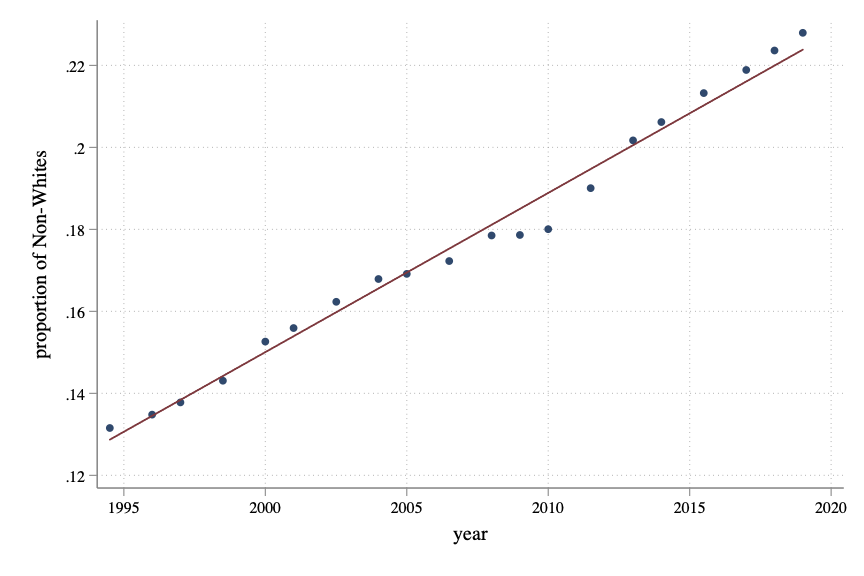
\includegraphics[width=\textwidth]{GraphNonWhites.png} 
\label{fig:1}
\end{figure}
\end{center}

\newpage

\begin{center}
\begin{figure}
\caption{Hispanics as a percentage of the total population in \\
the United States from 1995 to 2019.}
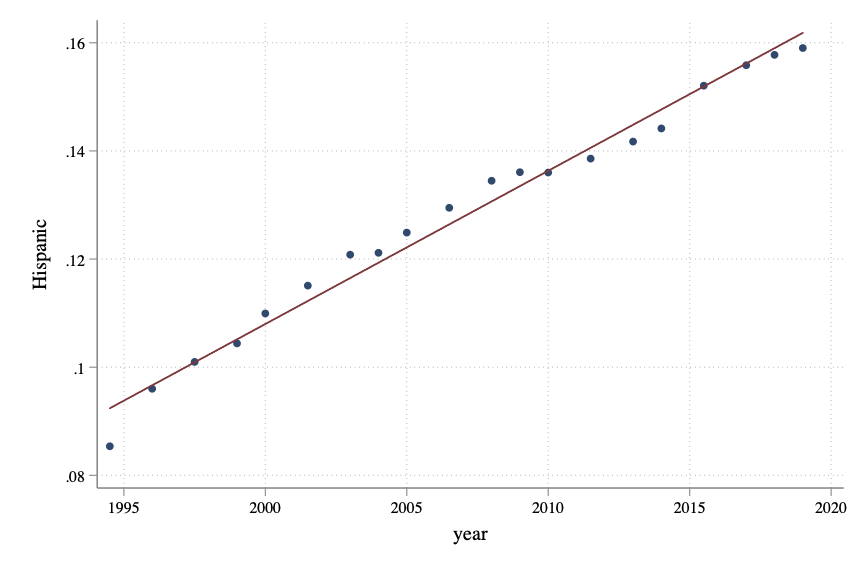
\includegraphics[width=\textwidth]{HispanicUSA.png} \label{fig:2}
\end{figure}
\end{center}

\newpage

\begin{center}
\begin{figure}
\caption{Inter-racial marriages as a percent of all marriages \\
 in the United States from 1995 to 2020.}
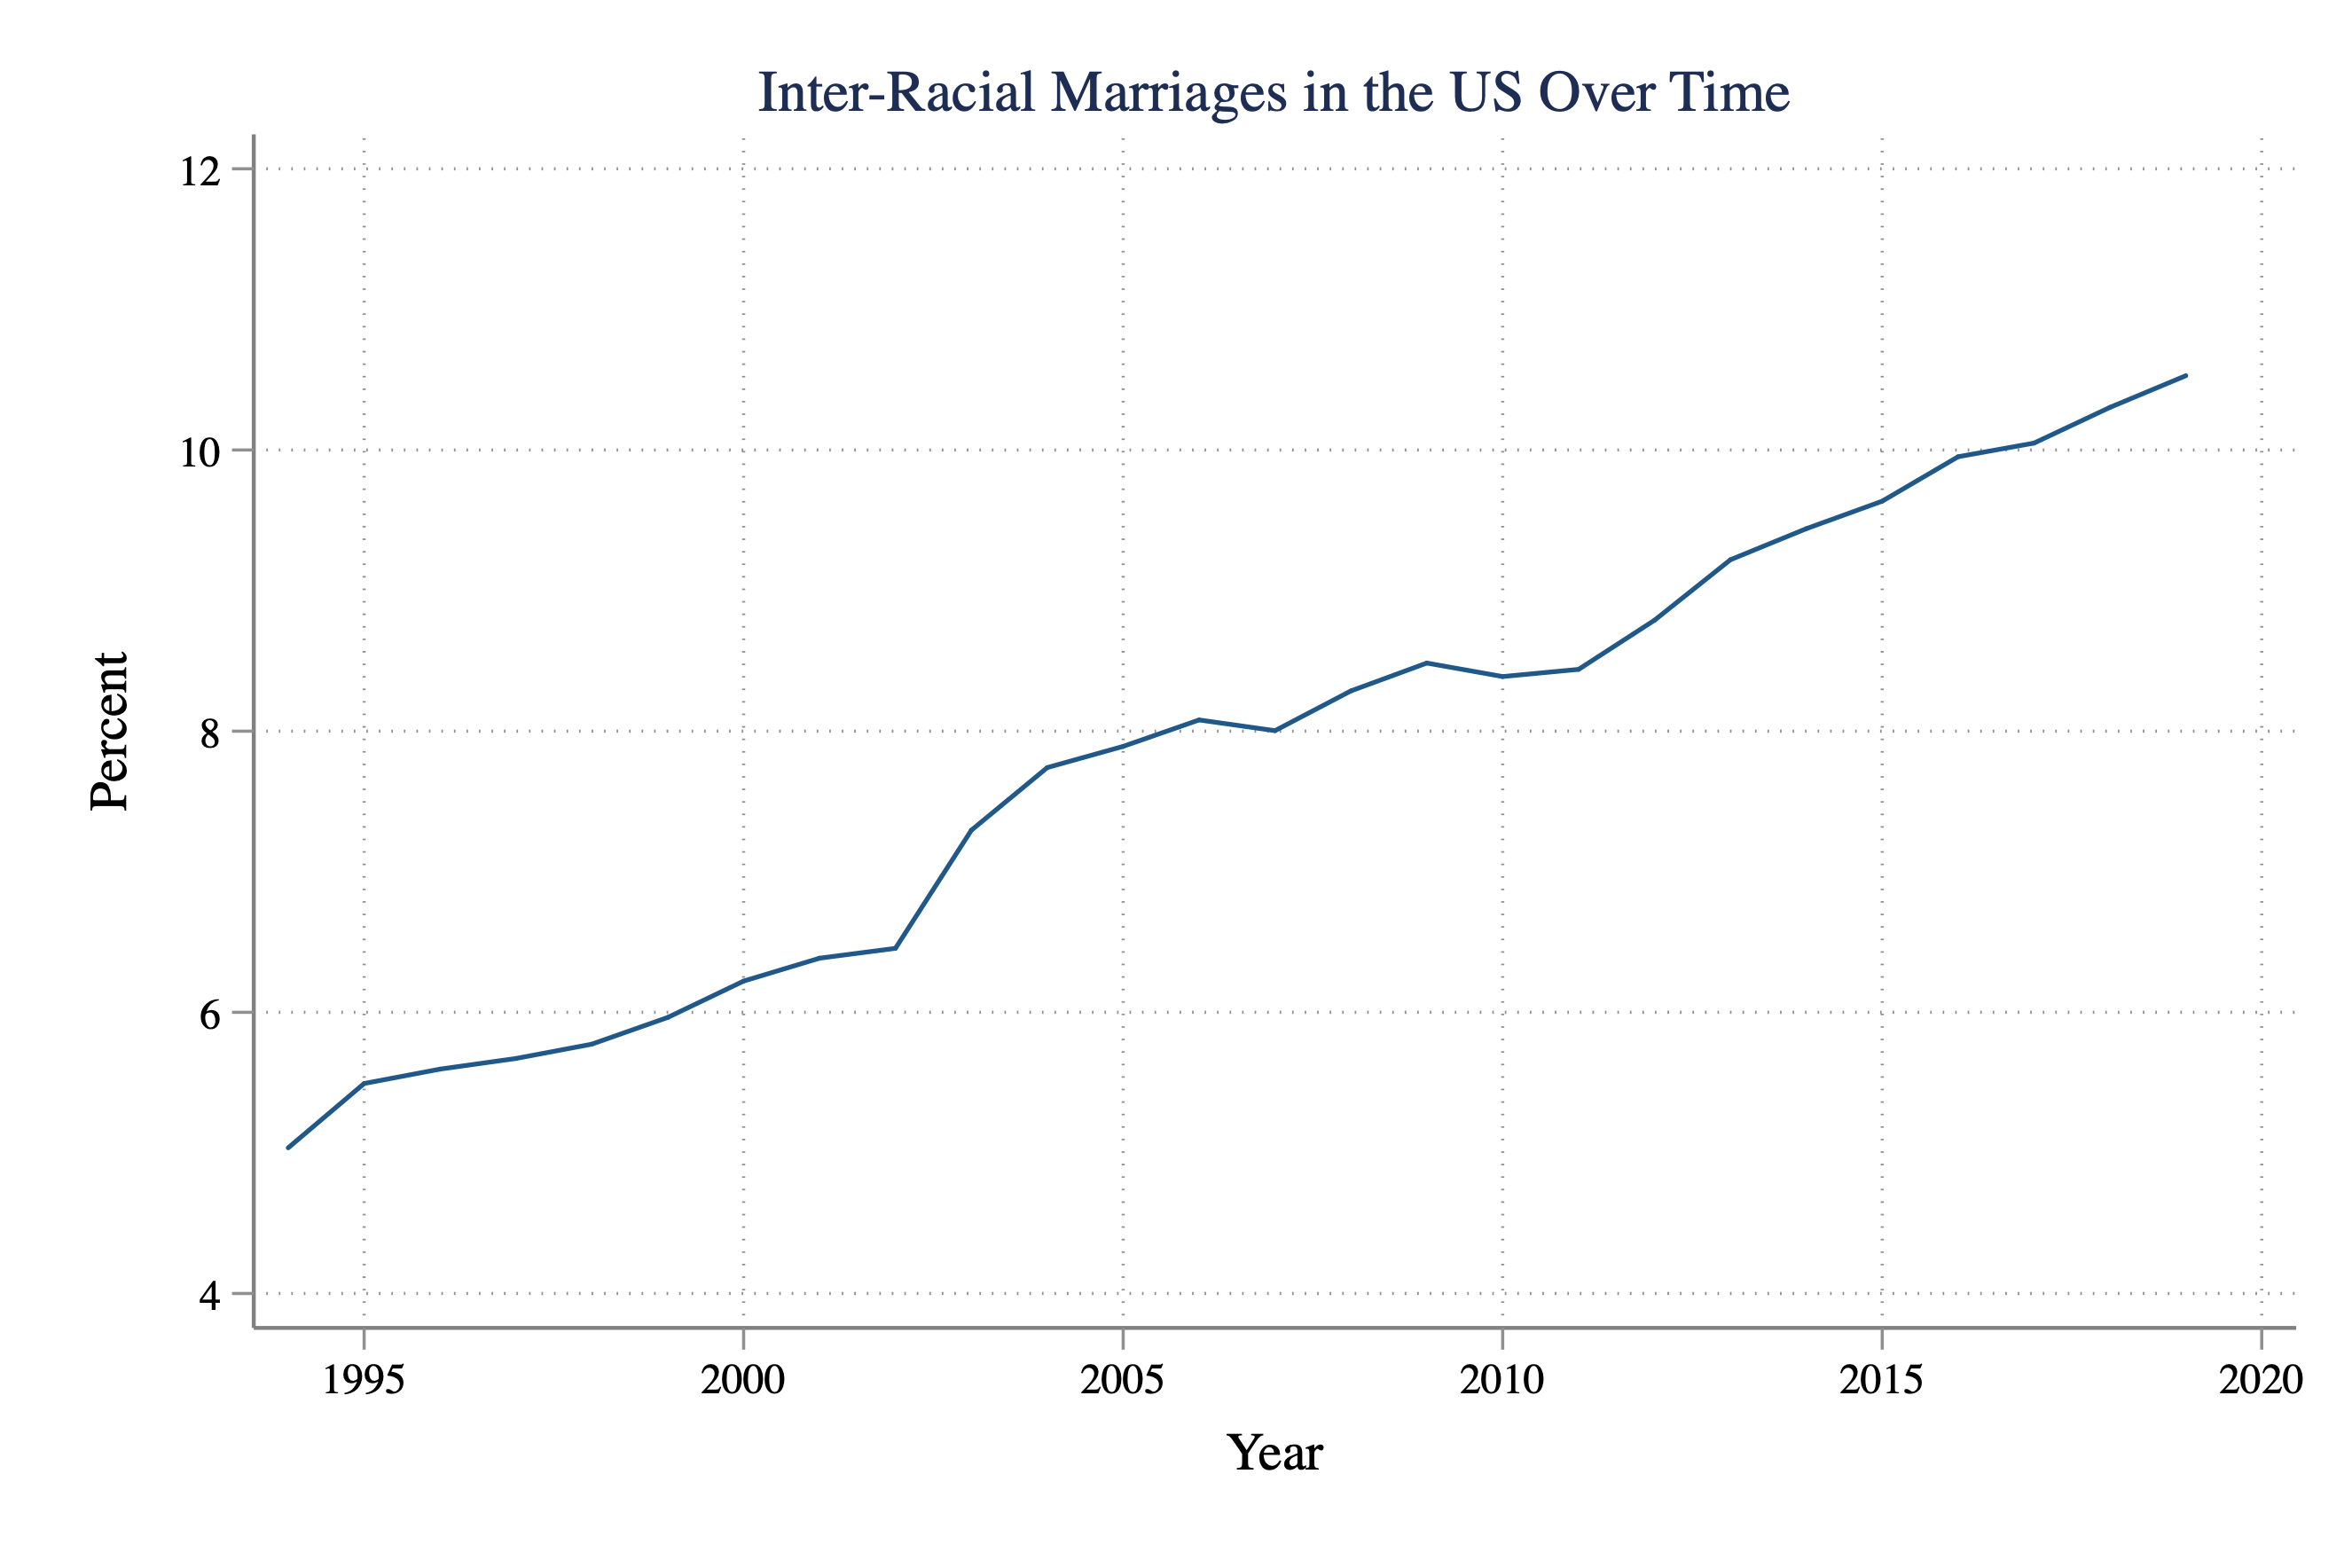
\includegraphics[width=\textwidth]{interracialovertime.png} 
\label{fig:3}
\end{figure}
\end{center}

\newpage

\begin{center}
\begin{figure}
\caption{Distribution of the four types of children.}
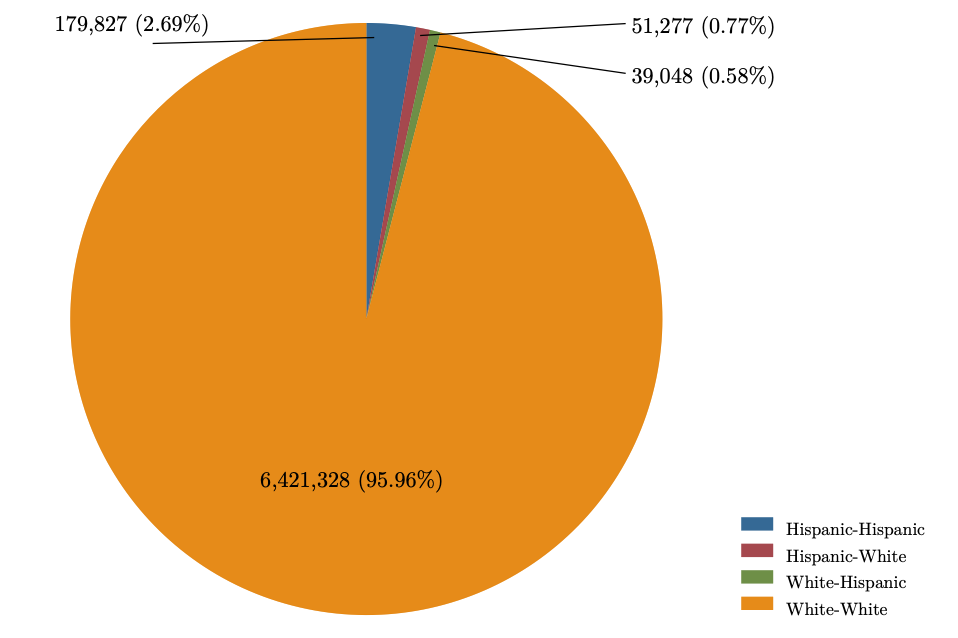
\includegraphics[width=\textwidth]{PirChart2.png} 
\label{fig:dist}
\end{figure}
\end{center}

\newpage
\begin{center}
\begin{figure}
\caption{Chart explaining which synthetic parents and children \\
and when we observe them.}
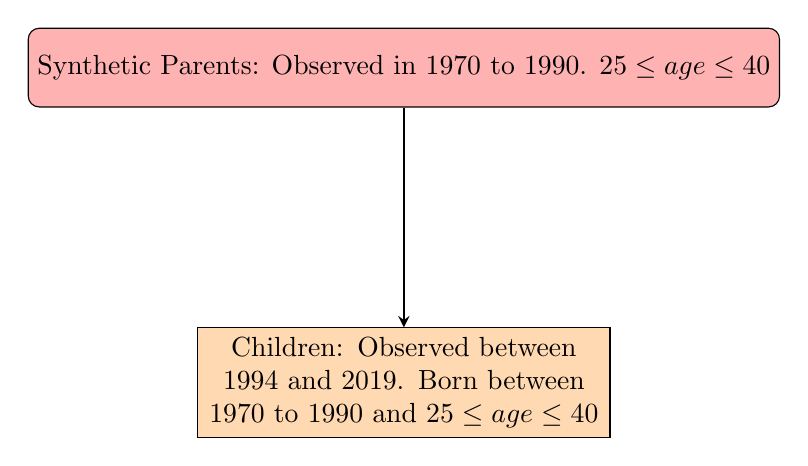
\begin{tikzpicture}[node distance =2cm]
\node (start) [startstop] {Synthetic Parents: Observed in 1970 to 1990. $25 \leq age \leq 40$};

\node (pro1) [process, below of = start, yshift = -2cm] {Children: Observed between 1994 and 2019. Born between 1970 to 1990 and $25 \leq age \leq 40$};

\draw [arrow] (start) -- (pro1);
\end{tikzpicture}
\label{flowchart1}
\end{figure}
\end{center}

\newpage

\section{tables}\label{appendix:tables}

\begin{table}[t]
\tablefont
\caption{Number of Children by Parental Type \label{tab:mat1}}
%\resizebox{\linewidth}{!}{
\begin{threeparttable}
\begin{tabular}[t]{>{}lcccc}
\toprule
\multicolumn{1}{c}{ } & \multicolumn{4}{c}{Perental Type} \\
\cmidrule(l{3pt}r{3pt}){2-5}
  & \specialcell{White Father \\ White Mother} & \specialcell{White Father \\ Hispanic Mother} & \specialcell{Hispanic Father \\ White Mother} & \specialcell{Hispanic Father \\ Hispanic Mother}\\
\midrule
\textbf{\specialcell{Observations\\Share}} & \specialcell{6,421,328\\0.96} & \specialcell{39,048\\0.01} & \specialcell{51,277\\0.01} & \specialcell{179,827\\0.03}\\
\bottomrule
\end{tabular}
\begin{tablenotes}
\item[1] Source: Current Population Surveys (CPS) 1994-2019
\item[2] The sample includes Whites, who are married, and are between the ages 25 and 40. Ethnicity of a person's parents are identified by the parent's place of birth. A parent is Hispanic if she/he was born in a Spanish-speaking country. A parent is White if she/he was born in the United States.
\end{tablenotes}
\end{threeparttable}
%}
\end{table}


% \begin{table}[H]
%   \centering
%   \renewcommand*\TPTnoteLabel[1]{\parbox[b]{3em}{\hfill#1\,}}
%   \begin{adjustbox}{max width=\textwidth}
%   \begin{threeparttable}
% \caption{\textsc{Number of children from the different types of parents.}}\label{tab:mat1}
% \footnotesize
% \begin{tabular}{cccccccccccccc}
% \hline 
%  &  &  & \multicolumn{10}{c}{Perent's Type} & \tabularnewline
% \cline{4-13} 
%  &  &  & White Father &  &  & White Father &  &  & Hispanic father &  &  & Hispanic father & \tabularnewline
%  &  &  & White Mother &  &  & Hispanic Mother &  &  & White Mother &  &  & Hispanic Mother & \tabularnewline
% \hline 
%  &  &  &  &  &  &  &  &  &  &  &  &  & \tabularnewline
%  & Number &  & 3,828,024 &  &  & 24,306 &  &  & 35,841 &  &  & 135,300 & \tabularnewline
%  & (\%) &  & (95.14\%) &  &  & (0.89\%) &  &  & (0.89\%) &  &  & (3.36\%) & \tabularnewline
%  &  &  &  &  &  &  &  &  &  &  &  &  & \tabularnewline
% \hline 
% \end{tabular}
%  \begin{tablenotes}
%    \item [\textit{Notes.}] The data is restricted to people interviewed between 1994 and 2019, also White, married, and between the ages of 18 and 65. I identify the ethnicity of a person's parents through the parent's place of birth. A parent is Hispanic if both her parents were born in a Spanish-speaking country. A parent is White if born parents were born in the United States.
%   \end{tablenotes}
%   \end{threeparttable}
%   \end{adjustbox}
% \end{table}

\newpage

\begin{table}[!h]

\caption{Couples' Type \label{tab:mat2}}
\centering
\resizebox{\linewidth}{!}{
\begin{threeparttable}
\begin{tabular}[t]{>{}lcccc}
\toprule
\multicolumn{1}{c}{ } & \multicolumn{4}{c}{Couples' Type} \\
\cmidrule(l{3pt}r{3pt}){2-5}
  & \specialcell{White Husband \\ White Wife} & \specialcell{White Husband \\ Hispanic Wife} & \specialcell{Hispanic Husband \\ White Wife} & \specialcell{Hispanic Husband \\ Hispanic Wife}\\
\midrule
\textbf{Observations} & \specialcell{1,286,731\\(0.97)} & \specialcell{7,178\\(0.01)} & \specialcell{7,606\\(0.01)} & \specialcell{20,911\\(0.02)}\\
\bottomrule
\end{tabular}
\begin{tablenotes}
\item[1] The data is restricted to people interviewed in 1970 and 1960 and also White and married. I identify the ethnicity of a person through their place of birth. A parent is Hispanic if they were born in a Spanish-speaking country. A parent is White if they were born in the United States.
\item[2] The table includes information on the proportion of the four types of synthetic parents that I have constructed.
\end{tablenotes}
\end{threeparttable}}
\end{table}


% \begin{table}[H]
% \begin{adjustbox}{max width=\textwidth}
%   \centering
%   \renewcommand*\TPTnoteLabel[1]{\parbox[b]{3em}{\hfill#1\,}}
%   \begin{threeparttable}
% \caption{\textsc{Parents' types}}\label{tab:mat2}
% \footnotesize
% \begin{tabular}{cccccccccccccc}
% \hline 
%  &  &  & \multicolumn{10}{c}{Couples' Type} & \tabularnewline
% \cline{4-13} 
%  &  &  & White Husband &  &  & White Husband &  &  & Hispanic Husband &  &  & Hispanic Husband & \tabularnewline
%  &  &  & White Wife &  &  & Hispanic Wife &  &  & White Wife &  &  & Hispanic Wife & \tabularnewline
% \hline 
%  &  &  &  &  &  &  &  &  &  &  &  &  & \tabularnewline
%  & Number &  & 1,198,446 &  &  & 3,819 &  &  & 3,413 &  &  & 6,920 & \tabularnewline
%  & (\%) &  & (98.83\%) &  &  & (0.31\%) &  &  & (0.28\%) &  &  & (0.57\%) & \tabularnewline
%  &  &  &  &  &  &  &  &  &  &  &  &  & \tabularnewline
% \hline 
% \end{tabular}

%   \begin{tablenotes}
%     \item [\textit{Notes.}] The data is restricted to people interviewed in 1970 and 1960 and also White and married. I identify the ethnicity of a person through their place of birth. A parent is Hispanic if they were born in a Spanish-speaking country. A parent is White if they were born in the United States.
%     \item [\textit{Notes.}] The table includes information on the proportion of the four types of synthetic parents that I have constructed.
%   \end{tablenotes}
%   \end{threeparttable}
% \end{adjustbox}
% \end{table}


\newpage

\begin{table}[!h]

\caption{Summary statistics of outcomes using parent's place of birth \label{tab:c&p1}}
\centering
\resizebox{\linewidth}{!}{
\begin{threeparttable}
\begin{tabular}[t]{lcccccc}
\toprule
\multicolumn{1}{c}{ } & \multicolumn{4}{c}{Father's and Mother's Ethnicities} & \multicolumn{2}{c}{Differences} \\
\cmidrule(l{3pt}r{3pt}){2-5} \cmidrule(l{3pt}r{3pt}){6-7}
Variables & \specialcell{White Father \\ White Mother \\ (WW) \\ (i)} & \specialcell{White Father \\ Hispanic Mother \\ (WH) \\ (ii)} & \specialcell{Hispanic Father \\ White Mother \\ (HW) \\ (iii)} & \specialcell{Hispanic Father \\ Hispanic Mother \\ (HH) \\ (iv)} & \specialcell{HH - WW \\ (v)} & \specialcell{HW - WH \\ (vi)}\\
\midrule
\textbf{Panel A: Parent’s} & \textbf{} & \textbf{} & \textbf{} & \textbf{} & \textbf{} & \textbf{}\\
\hspace{1em}Husband’seducation (Total Years) & \specialcell{13.05\\(2.44)} & \specialcell{12.32\\(3.33)} & \specialcell{10.65\\(4.39)} & \specialcell{8.93\\(4.41)} & \specialcell{-4.11**\\(0.02)} & \specialcell{-1.67**\\(0.04)}\\
\hspace{1em}Wife’seducation (Total Years) & \specialcell{12.74\\(2.12)} & \specialcell{11.03\\(3.92)} & \specialcell{11.54\\(3.12)} & \specialcell{8.6\\(4.13)} & \specialcell{-4.13**\\(0.02)} & \specialcell{0.51**\\(0.04)}\\
\hspace{1em}Total Household seducation (Total Years) & \specialcell{25.78\\(4.08)} & \specialcell{23.35\\(6.51)} & \specialcell{22.19\\(6.69)} & \specialcell{17.54\\(7.83)} & \specialcell{-8.25**\\(0.03)} & \specialcell{-1.16*\\(0.07)}\\
\textbf{Panel B: Education} & \textbf{} & \textbf{} & \textbf{} & \textbf{} & \textbf{} & \textbf{}\\
\addlinespace
\hspace{1em}Men’s education (Total Years) & \specialcell{13.91\\(2.39)} & \specialcell{13.58\\(2.35)} & \specialcell{13.21\\(2.32)} & \specialcell{12.91\\(2.26)} & \specialcell{-1.00***\\(0.01)} & \specialcell{-0.36**\\(0.03)}\\
\hspace{1em}Women’s education (Total Years) & \specialcell{14.29\\(2.41)} & \specialcell{13.87\\(2.47)} & \specialcell{13.42\\(2.35)} & \specialcell{13.27\\(2.37)} & \specialcell{-1.01***\\(0.01)} & \specialcell{-0.46**\\(0.03)}\\
\textbf{Panel C: Employment and Earnings} & \textbf{} & \textbf{} & \textbf{} & \textbf{} & \textbf{} & \textbf{}\\
\hspace{1em}Men’s Employment Rate & \specialcell{0.95\\(0.22)} & \specialcell{0.94\\(0.23)} & \specialcell{0.92\\(0.26)} & \specialcell{0.93\\(0.26)} & \specialcell{-0.02***\\(0.00)} & \specialcell{-0.02***\\(0.00)}\\
\hspace{1em}Women’s Employment Rate & \specialcell{0.96\\(0.2)} & \specialcell{0.95\\(0.22)} & \specialcell{0.93\\(0.25)} & \specialcell{0.94\\(0.24)} & \specialcell{-0.02***\\(0.00)} & \specialcell{-0.02***\\(0.00)}\\
\addlinespace
\hspace{1em}Men’s Log Hourly Earnings & \specialcell{2.48\\(0.45)} & \specialcell{2.41\\(0.45)} & \specialcell{2.4\\(0.44)} & \specialcell{2.41\\(0.43)} & \specialcell{-0.07***\\(0.01)} & \specialcell{-0.00**\\(0.02)}\\
\hspace{1em}Women’s Hourly Earnings & \specialcell{2.33\\(0.49)} & \specialcell{2.33\\(0.46)} & \specialcell{2.27\\(0.45)} & \specialcell{2.3\\(0.41)} & \specialcell{-0.02***\\(0.01)} & \specialcell{-0.06**\\(0.02)}\\
\hspace{1em}Men’s Log Annual Earnings & \specialcell{10.25\\(1.01)} & \specialcell{10.08\\(1.05)} & \specialcell{10.04\\(1.06)} & \specialcell{10.01\\(1.04)} & \specialcell{-0.25**\\(0.01)} & \specialcell{-0.04**\\(0.03)}\\
\hspace{1em}Women’s Hourly Earnings & \specialcell{9.46\\(1.78)} & \specialcell{9.54\\(1.64)} & \specialcell{9.47\\(1.57)} & \specialcell{9.53\\(1.52)} & \specialcell{0.07**\\(0.02)} & \specialcell{-0.07*\\(0.06)}\\
\textbf{Panel D: Hispanic Identity} & \textbf{} & \textbf{} & \textbf{} & \textbf{} & \textbf{} & \textbf{}\\
\addlinespace
\hspace{1em}Men & \specialcell{0.05} & \specialcell{0.81} & \specialcell{0.88} & \specialcell{0.97} &  & \\
\hspace{1em}Women & \specialcell{0.06} & \specialcell{0.85} & \specialcell{0.87} & \specialcell{0.97} &  & \\
\bottomrule
\end{tabular}
\begin{tablenotes}
\item[1] The data is restricted to native-born United States citizens between 1994 and 2019 who are also White and between the ages of 25 and 40. I identify the ethnicity of a person's parents through the parent's place of birth. A parent is Hispanic if they were born in a Spanish-speaking country. A parent is White if they were born in the United States.
\item[2] In each column, I present the average statistics of the different types of people based on the ethnicities of their parents. In column one, I show the summary statistics of children of White fathers and White mothers. In column two, I present the summary statistics of children of White fathers and Hispanic mothers. In column three, I show the summary statistics of children of Hispanic fathers and White mothers. In column four, I present the summary statistics of children of Hispanic fathers and mothers.
\item[3] Columns five and six have data on the HH--WW gaps (column five) and the HW--WH gaps (column six).
\end{tablenotes}
\end{threeparttable}}
\end{table}


% \newpage

% \begin{table}[H]
%   \centering
%   \renewcommand*\TPTnoteLabel[1]{\parbox[b]{3em}{\hfill#1\,}}
%   \begin{adjustbox}{max width=\textwidth}
%   \begin{threeparttable}
% \caption{\textsc{Children's outcome using parent's place of birth}}\label{tab:c&p1}
% \footnotesize
% \begin{tabular}{llccccccccr@{\extracolsep{0pt}.}l}
% \toprule 
%  &  & \multicolumn{4}{c}{Father's and Mother's Ethnicities} &  & \multicolumn{5}{c}{Differences}\tabularnewline
% \cmidrule{3-6} \cmidrule{8-12} 
%  &  &  &  &  &  &  &  &  &  & \multicolumn{2}{c}{}\tabularnewline
% Variables &  & White Father & White Father & Hispanic Father & Hispanic Father &  & HH - WW &  & HW-WH & \multicolumn{2}{c}{}\tabularnewline
%  &  & White Mother & Hispanic Mother & White Mother & Hispanic Mother &  &  &  &  & \multicolumn{2}{c}{}\tabularnewline
%  &  & (WW) & (WH) & (HW) & (HH) &  &  &  &  & \multicolumn{2}{c}{}\tabularnewline
%  &  & (i) & (ii) & (iii) & (iv) &  & (v) &  & (vi) & \multicolumn{2}{c}{}\tabularnewline
% \midrule
% \textbf{Parent's Panel:} &  &  &  &  &  &  &  &  &  & \multicolumn{2}{c}{}\tabularnewline
% Husband's education (total years) &  & 12.727 & 11.847 & 10.286 & 8.949 &  & -3.779{*}{*}{*} &  & -1.560{*}{*}{*} & \multicolumn{2}{c}{}\tabularnewline
%  &  & (2.616) & (3.658) & (4.602) & (4.422) &  & (0.018) &  & (0.041) & \multicolumn{2}{c}{}\tabularnewline
% Wife's education (total years) &  & 12.467 & 10.462 & 11.188 & 8.590 &  & -3.876{*}{*}{*} &  & 0.726{*}{*}{*} & \multicolumn{2}{c}{}\tabularnewline
%  &  & (2.182) & (4.139) & (3.394) & (4.120) &  & (0.015) &  & (0.035) & \multicolumn{2}{c}{}\tabularnewline
% Total Household education (years) &  & 25.194 & 22.308 & 21.473 & 17.539 &  & -7.655{*}{*}{*} &  & -0.835{*}{*}{*} & \multicolumn{2}{c}{}\tabularnewline
%  &  & (4.300) & (7.034) & (7.202) & (7.836) &  & (0.029) &  & (0.068) & \multicolumn{2}{c}{}\tabularnewline
% \textbf{Panel A:} &  &  &  &  &  &  &  &  &  & \multicolumn{2}{c}{}\tabularnewline
% \textbf{age and education} &  &  &  &  &  &  &  &  &  & \multicolumn{2}{c}{}\tabularnewline
% man's Education &  & 13.861 & 13.366 & 13.072 & 12.898 &  & -0.962{*}{*}{*} &  & -0.294{*}{*}{*} & \multicolumn{2}{c}{}\tabularnewline
%  &  & (2.421) & (2.317) & (2.270) & (2.356) &  &  &  &  & \multicolumn{2}{c}{}\tabularnewline
% woman's Education &  & 14.200 & 13.741 & 13.270 & 13.204 &  & -0.996{*}{*}{*} &  & -0.471{*}{*}{*} & \multicolumn{2}{c}{}\tabularnewline
%  &  & (2.424) & (2.467) & (2.342) & (2.453) &  &  &  &  & \multicolumn{2}{c}{}\tabularnewline
% \textbf{Panel B: Employment \& Earnings} &  &  &  &  &  &  &  &  &  & \multicolumn{2}{c}{}\tabularnewline
% men' employment rate &  & 0.952 & 0.945 & 0.927 & 0.931 &  & -0.021{*}{*}{*} &  & -0.018{*}{*}{*} & \multicolumn{2}{c}{}\tabularnewline
%  &  & (0.215) & (0.227) & (0.260) & (0.254) &  &  &  &  & \multicolumn{2}{c}{}\tabularnewline
% women' employment rate &  & 0.956 & 0.950 & 0.931 & 0.936 &  & -0.020{*}{*}{*} &  & -0.019{*}{*}{*} & \multicolumn{2}{c}{}\tabularnewline
%  &  & (0.205) & (0.218) & (0.253) & (0.244) &  &  &  &  & \multicolumn{2}{c}{}\tabularnewline
% men' log hourly earnings &  & 2.557 & 2.524 & 2.468 & 2.505 &  & -0.041{*}{*}{*} &  & -0.056{*}{*}{*} & \multicolumn{2}{c}{}\tabularnewline
%  &  & (0.399) & (0.421) & (0.423) & (0.401) &  &  &  &  & \multicolumn{2}{c}{}\tabularnewline
% women' log hourly earnings &  & 2.435 & 2.444 & 2.385 & 2.389 &  & -0.016{*}{*} &  & -0.061{*}{*}{*} & \multicolumn{2}{c}{}\tabularnewline
%  &  & (0.415) & (0.426) & (0.375) & (0.376) &  &  &  &  & \multicolumn{2}{c}{}\tabularnewline
% men' log annual earnings &  & 10.529 & 10.435 & 10.386 & 10.365 &  & -0.164{*}{*}{*} &  & -0.049 & \multicolumn{2}{c}{}\tabularnewline
%  &  & (0.703) & (0.637) & (0.872) & (0.622) &  &  &  &  & \multicolumn{2}{c}{}\tabularnewline
% women' log annual earnings &  & 10.297 & 10.262 & 10.159 & 10.175 &  & -0.123{*}{*}{*} &  & -0.103{*}{*}{*} & \multicolumn{2}{c}{}\tabularnewline
%  &  & (0.633) & (0.613) & (0.541) & (0.650) &  &  &  &  & \multicolumn{2}{c}{}\tabularnewline
% \textbf{Panel D: Identity} &  &  &  &  &  &  &  &  &  & \multicolumn{2}{c}{}\tabularnewline
% Proportion of men &  & 0.060 & 0.821 & 0.879 & 0.969 &  &  &  &  & \multicolumn{2}{c}{}\tabularnewline
% identifying as Hispanic &  &  &  &  &  &  &  &  &  & \multicolumn{2}{c}{}\tabularnewline
% Proportion of women &  & 0.059 & 0.850 & 0.859 & 0.970 &  &  &  &  & \multicolumn{2}{c}{}\tabularnewline
% identifying as Hispanic &  &  &  &  &  &  &  &  &  & \multicolumn{2}{c}{}\tabularnewline
%  &  &  &  &  &  &  &  &  &  & \multicolumn{2}{c}{}\tabularnewline
% \bottomrule
% \end{tabular}
%   \begin{tablenotes}
%    \item [\textit{Notes.}] The data is restricted to native-born United States citizens between 1994 and 2019 who are also White and between the ages of 25 and 40. I identify the ethnicity of a person's parents through the parent's place of birth. A parent is Hispanic if they were born in a Spanish-speaking country. A parent is White if they were born in the United States.
%    \item [\textit{Notes.}] In each column, I present the average statistics of the different types of people based on the ethnicities of their parents. In column one, I show the summary statistics of children of White fathers and White mothers. In column two, I present the summary statistics of children of White fathers and Hispanic mothers. In column three, I show the summary statistics of children of Hispanic fathers and White mothers. In column four, I present the summary statistics of children of Hispanic fathers and mothers.
%    \item [\textit{Notes.}] Columns five and six have data on the HH--WW gaps (column five) and the HW--WH gaps (column six).

%   \end{tablenotes}
%   \end{threeparttable}
%   \end{adjustbox}
% \end{table}

\newpage

\begin{table}[!h]

\caption{Summary statistics of outcomes using parent's place of birth only for those that self-identify as Hispanic \label{tab:c&p2}}
\centering
\resizebox{\linewidth}{!}{
\begin{threeparttable}
\begin{tabular}[t]{lcccccc}
\toprule
\multicolumn{1}{c}{ } & \multicolumn{4}{c}{Father's and Mother's Ethnicities} & \multicolumn{2}{c}{Differences} \\
\cmidrule(l{3pt}r{3pt}){2-5} \cmidrule(l{3pt}r{3pt}){6-7}
Variables & \specialcell{White Father \\ White Mother \\ (WW) \\ (i)} & \specialcell{White Father \\ Hispanic Mother \\ (WH) \\ (ii)} & \specialcell{Hispanic Father \\ White Mother \\ (HW) \\ (iii)} & \specialcell{Hispanic Father \\ Hispanic Mother \\ (HH) \\ (iv)} & \specialcell{HH - WW \\ (v)} & \specialcell{HW - WH \\ (vi)}\\
\midrule
\textbf{Panel A: Parent’s} & \textbf{} & \textbf{} & \textbf{} & \textbf{} & \textbf{} & \textbf{}\\
\hspace{1em}Husband’seducation (Total Years) & \specialcell{13.05\\(2.44)} & \specialcell{12.32\\(3.33)} & \specialcell{10.65\\(4.39)} & \specialcell{8.93\\(4.41)} & \specialcell{-4.11\\(0.02)} & \specialcell{-1.67\\(0.04)}\\
\hspace{1em}Wife’seducation (Total Years) & \specialcell{12.74\\(2.12)} & \specialcell{11.03\\(3.92)} & \specialcell{11.54\\(3.12)} & \specialcell{8.6\\(4.13)} & \specialcell{-4.13\\(0.02)} & \specialcell{0.51\\(0.04)}\\
\hspace{1em}Total Household seducation (Total Years) & \specialcell{25.78\\(4.08)} & \specialcell{23.35\\(6.51)} & \specialcell{22.19\\(6.69)} & \specialcell{17.54\\(7.83)} & \specialcell{-8.25\\(0.03)} & \specialcell{-1.16\\(0.07)}\\
\textbf{Panel B: Education} & \textbf{} & \textbf{} & \textbf{} & \textbf{} & \textbf{} & \textbf{}\\
\addlinespace
\hspace{1em}Men’s education (Total Years) & \specialcell{12.97\\(2.15)} & \specialcell{13.45\\(2.37)} & \specialcell{13.13\\(2.27)} & \specialcell{12.89\\(2.25)} & \specialcell{-0.08\\(0.01)} & \specialcell{-0.32\\(0.03)}\\
\hspace{1em}Women’s education (Total Years) & \specialcell{13.23\\(2.25)} & \specialcell{13.75\\(2.41)} & \specialcell{13.32\\(2.34)} & \specialcell{13.26\\(2.37)} & \specialcell{0.03\\(0.01)} & \specialcell{-0.43\\(0.03)}\\
\textbf{Panel C: Employment and Earnings} & \textbf{} & \textbf{} & \textbf{} & \textbf{} & \textbf{} & \textbf{}\\
\hspace{1em}Men’s Employment Rate & \specialcell{0.93\\(0.26)} & \specialcell{0.94\\(0.23)} & \specialcell{0.92\\(0.27)} & \specialcell{0.93\\(0.26)} & \specialcell{0.00\\(0.00)} & \specialcell{-0.02\\(0.00)}\\
\hspace{1em}Women’s Employment Rate & \specialcell{0.94\\(0.25)} & \specialcell{0.94\\(0.23)} & \specialcell{0.93\\(0.26)} & \specialcell{0.94\\(0.24)} & \specialcell{0.00\\(0.00)} & \specialcell{-0.02\\(0.00)}\\
\addlinespace
\hspace{1em}Men’s Log Hourly Earnings & \specialcell{2.4\\(0.44)} & \specialcell{2.41\\(0.45)} & \specialcell{2.4\\(0.44)} & \specialcell{2.41\\(0.43)} & \specialcell{0.01\\(0.01)} & \specialcell{-0.01\\(0.02)}\\
\hspace{1em}Women’s Hourly Earnings & \specialcell{2.26\\(0.43)} & \specialcell{2.32\\(0.45)} & \specialcell{2.27\\(0.45)} & \specialcell{2.3\\(0.41)} & \specialcell{0.04\\(0.01)} & \specialcell{-0.05\\(0.02)}\\
\hspace{1em}Men’s Log Annual Earnings & \specialcell{10.02\\(1.02)} & \specialcell{10.06\\(1.06)} & \specialcell{10.03\\(0.99)} & \specialcell{10\\(1.04)} & \specialcell{-0.02\\(0.01)} & \specialcell{-0.03\\(0.04)}\\
\hspace{1em}Women’s Hourly Earnings & \specialcell{9.44\\(1.59)} & \specialcell{9.55\\(1.59)} & \specialcell{9.47\\(1.55)} & \specialcell{9.52\\(1.52)} & \specialcell{0.08\\(0.02)} & \specialcell{-0.08\\(0.05)}\\
\bottomrule
\end{tabular}
\begin{tablenotes}
\item[1] The data is restricted to native-born United States citizens between 1994 and 2019 who are also White and between the ages of 25 and 40. I identify the ethnicity of a person's parents through the parent's place of birth. A parent is Hispanic if they were born in a Spanish-speaking country. A parent is White if they were born in the United States.
\item[2] In each column, I present the average statistics of the different types of people based on the ethnicities of their parents. In column one, I show the summary statistics of children of White fathers and White mothers. In column two, I present the summary statistics of children of White fathers and Hispanic mothers. In column three, I show the summary statistics of children of Hispanic fathers and White mothers. In column four, I present the summary statistics of children of Hispanic fathers and mothers.
\item[3] Columns five and six have data on the HH--WW gaps (column five) and the HW--WH gaps (column six).
\end{tablenotes}
\end{threeparttable}}
\end{table}


% \begin{table}[H]
%   \centering
%   \renewcommand*\TPTnoteLabel[1]{\parbox[b]{3em}{\hfill#1\,}}
%   \begin{adjustbox}{max width=\textwidth}
%   \begin{threeparttable}
% \caption{\textsc{Children's outcomes using parent's place of birth only for those that identify as Hispanic}}\label{tab:c&p2}
% \footnotesize
% \begin{tabular}{llccccccccr@{\extracolsep{0pt}.}l}
% \hline 
%  &  & \multicolumn{4}{c}{Father's and Mother's Ethnicities} &  & \multicolumn{5}{c}{Differences}\tabularnewline
% \cline{3-6} \cline{8-12} 
%  &  &  &  &  &  &  &  &  &  & \multicolumn{2}{c}{}\tabularnewline
% Variables &  & White Father & White Father & Hispanic Father & Hispanic Father &  & HH - WW &  & HW-WH & \multicolumn{2}{c}{}\tabularnewline
%  &  & White Mother & Hispanic Mother & White Mother & Hispanic Mother &  &  &  &  & \multicolumn{2}{c}{}\tabularnewline
%  &  & (WW) & (WH) & (HW) & (HH) &  &  &  &  & \multicolumn{2}{c}{}\tabularnewline
%  &  & (i) & (ii) & (iii) & (iv) &  & (v) &  & (vi) & \multicolumn{2}{c}{}\tabularnewline
% \hline 
% \textbf{Parent's Panel:} &  &  &  &  &  &  &  &  &  & \multicolumn{2}{c}{}\tabularnewline
% Husband's education (total years) &  & 11.856 & 10.211 & 9.665 & 8.427 &  & -3.429{*}{*}{*} &  & -0.546{*}{*}{*} & \multicolumn{2}{c}{}\tabularnewline
%  &  & (2.922) & (3.876) & (4.095) & (4.228) &  & (0.035) &  & (0.079) & \multicolumn{2}{c}{}\tabularnewline
% Wife's education (total years) &  & 11.793 & 9.556 & 9.791 & 8.137 &  & -3.656{*}{*}{*} &  & 0.235{*}{*}{*} & \multicolumn{2}{c}{}\tabularnewline
%  &  & (2.329) & (3.751) & (3.524) & (3.899) &  & (0.028) &  & (0.063) & \multicolumn{2}{c}{}\tabularnewline
% Total Household education (years) &  & 23.650 & 19.767 & 19.456 & 16.564 &  & -7.085{*}{*}{*} &  & -0.311{*}{*}{*} & \multicolumn{2}{c}{}\tabularnewline
%  &  & (4.716) & (6.843) & (6.896) & (7.338) &  & (0.057) &  & (0.128) & \multicolumn{2}{c}{}\tabularnewline
% \textbf{Panel A:} &  &  &  &  &  &  &  &  &  & \multicolumn{2}{c}{}\tabularnewline
% \textbf{age and education} &  &  &  &  &  &  &  &  &  & \multicolumn{2}{c}{}\tabularnewline
% man's Education &  & 13.861 & 13.237 & 13.008 & 12.874 &  & -0.986{*}{*}{*} &  & -0.230{*}{*}{*} & \multicolumn{2}{c}{}\tabularnewline
%  &  & (2.421) & (2.313) & (2.217) & (2.347) &  &  &  &  & \multicolumn{2}{c}{}\tabularnewline
% woman's Education &  & 14.200 & 13.603 & 13.133 & 13.182 &  & -1.018{*}{*}{*} &  & -0.470{*}{*}{*} & \multicolumn{2}{c}{}\tabularnewline
%  &  & (2.424) & (2.391) & (2.325) & (2.453) &  &  &  &  & \multicolumn{2}{c}{}\tabularnewline
% \textbf{Panel D: Employment \& Earnings} &  &  &  &  &  &  &  &  &  & \multicolumn{2}{c}{}\tabularnewline
% men' employment rate &  & 0.952 & 0.943 & 0.925 & 0.930 &  & -0.021{*}{*}{*} &  & -0.018{*}{*}{*} & \multicolumn{2}{c}{}\tabularnewline
%  &  & (0.215) & (0.232) & (0.264) & (0.254) &  &  &  &  & \multicolumn{2}{c}{}\tabularnewline
% women' employment rate &  & 0.956 & 0.948 & 0.928 & 0.936 &  & -0.020{*}{*}{*} &  & -0.020{*}{*}{*} & \multicolumn{2}{c}{}\tabularnewline
%  &  & (0.205) & (0.222) & (0.258) & (0.245) &  &  &  &  & \multicolumn{2}{c}{}\tabularnewline
% men' log hourly earnings &  & 2.501 & 2.470 & 2.408 & 2.460 &  & -0.041{*}{*}{*} &  & -0.062{*}{*}{*} & \multicolumn{2}{c}{}\tabularnewline
%  &  & (0.454) & (0.458) & (0.463) & (0.434) &  &  &  &  & \multicolumn{2}{c}{}\tabularnewline
% women' log hourly earnings &  & 2.339 & 2.358 & 2.288 & 2.322 &  & -0.017{*}{*} &  & -0.071{*}{*}{*} & \multicolumn{2}{c}{}\tabularnewline
%  &  & (0.494) & (0.499) & (0.464) & (0.423) &  &  &  &  & \multicolumn{2}{c}{}\tabularnewline
% men' log annual earnings &  & 10.529 & 10.414 & 10.394 & 10.364 &  & -0.165{*}{*}{*} &  & -0.020 & \multicolumn{2}{c}{}\tabularnewline
%  &  & (0.703) & (0.610) & (0.704) & (0.625) &  &  &  &  & \multicolumn{2}{c}{}\tabularnewline
% women' log annual earnings &  & 10.297 & 10.240 & 10.136 & 10.172 &  & -0.126{*}{*}{*} &  & -0.104{*}{*}{*} & \multicolumn{2}{c}{}\tabularnewline
%  &  & (0.634) & (0.635) & (0.537) & (0.652) &  &  &  &  & \multicolumn{2}{c}{}\tabularnewline
%  &  &  &  &  &  &  &  &  &  & \multicolumn{2}{c}{}\tabularnewline
% \hline 
% \end{tabular}
%   \begin{tablenotes}
%    \item [\textit{Notes.}] The data is restricted to native-born United States citizens between 1994 and 2019 who are also White and between the ages of 25 and 40. I identify the ethnicity of a person's parents through the parent's place of birth. A parent is Hispanic if they were born in a Spanish-speaking country. A parent is White if they were born in the United States.
%    \item [\textit{Notes.}] In each column, I present the average statistics of those that identify as Hispanic by the different types of people based on the ethnicities of their parents. In column one, I present the summary statistics of children of White fathers and White mothers. In column two, I show the summary statistics of children of White fathers and Hispanic mothers identifying as Hispanic. In column three, I present the summary statistics of children of Hispanic fathers and White mothers that identify as Hispanic. In column four, I show the summary statistics of children of Hispanic fathers and Hispanic mothers that identify as Hispanic.
%    \item [\textit{Notes.}] Columns five and six have data on the HH--WW gaps (column five) and the HW--WH gaps (column six).

%   \end{tablenotes}
%   \end{threeparttable}
%   \end{adjustbox}
% \end{table}

\newpage

\begin{table}[!h]

\caption{Effect of Having Hispanic Last Name \label{tab:lastnamereg}}
\centering
\resizebox{\linewidth}{!}{
\begin{threeparttable}
\begin{tabular}[t]{lcc}
\toprule
  & \specialcell{(1) \\ Log annual earnings} & \specialcell{(2) \\  Log annual earnings}\\
\midrule
$WH_{i}$ & \num{-0.14}*** & \num{-0.09}***\\
 & (\num{0.03}) & (\num{0.02})\\
$HW_{i}$ & \num{-0.20}*** & \num{-0.11}***\\
 & (\num{0.02}) & \vphantom{1} (\num{0.01})\\
$HH_{i}$ & \num{-0.24}*** & \num{-0.12}***\\
 & (\num{0.02}) & (\num{0.01})\\
\midrule
$HW_{i} - WH_{i}$ & -0.06** & -0.02\\
 & (0.03) & (0.02)\\
\midrule
Observations & \num{129359} & \num{129359}\\
State FE & X & X\\
Year FE & X & X\\
\textit{Controlling for:} &  & \\
Hours Worked & X & X\\
Age & X & X\\
Education &  & X\\
\bottomrule
\multicolumn{3}{l}{\rule{0pt}{1em}* p $<$ 0.1, ** p $<$ 0.05, *** p $<$ 0.01}\\
\end{tabular}
\begin{tablenotes}
\item[1] \footnotesize{This table includes the estimation results of equation (\ref{eq:1a}).}
\item[2] \footnotesize{The four groups stand for White Husband White Wife (WW), White Husband Hispanic Wife (WH), Hispanic Husband White (HW), and Hispanic Husband Hispanic Wife (HH).}
\item[3] \footnotesize{The sample is restricted to men working full-time full-year and are waged and salaried workers.}
\item[4] \footnotesize{Column one has the regression results when controlling for hours worked, age, and fixed effects. Column two has the results after controlling for education.}
\item[5] \footnotesize{Standard errors are clustered on the state level.}
\end{tablenotes}
\end{threeparttable}}
\end{table}


% \begin{table}[H]
%   \centering
%   \renewcommand*\TPTnoteLabel[1]{\parbox[b]{3em}{\hfill#1\,}}
%     \begin{adjustbox}{max width=\textwidth}
%   \begin{threeparttable}
% \caption{\textsc{Effect of having a Hispanic last name}}\label{tab:lastnamereg}
% \footnotesize

% \begin{tabular}{llcccc}
% \toprule 
%  &  &  &  &  & \tabularnewline
% Variables &  & Log annual earnings &  & Log annual earnings & \tabularnewline
% \midrule

% $WH_{ist}$ &  & -0.088{*}{*}{*} &  & -0.044{*}{*}{*} & \tabularnewline
%  &  & (0.018) &  & (0.017) & \tabularnewline
%  &  &  &  &  & \tabularnewline
% $HW_{ist}$ &  & -0.141{*}{*}{*} &  & -0.059{*}{*}{*} & \tabularnewline
%  &  & (0.015) &  & (0.014) & \tabularnewline
%  &  &  &  &  & \tabularnewline
% $HH_{ist}$ &  & -0.161{*}{*}{*} &  & -0.058{*}{*}{*} & \tabularnewline
%  &  & (0.008) &  & (0.007) & \tabularnewline
%  &  &  &  &  & \tabularnewline
% \midrule
% $HW_{ist}$ - $WH_{ist}$ &  & -0.053{*}{*} &  & -0.016 & \tabularnewline
%  &  & (0.024) &  & (0.022) & \tabularnewline
%  &  &  &  &  & \tabularnewline
% \midrule
% \textit{Controlling for:} &  &  &  &  & \tabularnewline
% Education &  & No &  & Yes & \tabularnewline
% Hours worked &  & Yes &  & Yes & \tabularnewline
% Age &  & Yes &  & Yes & \tabularnewline
% Year FE &  & Yes &  & Yes & \tabularnewline
% \bottomrule
% \end{tabular}


%   \begin{tablenotes}
%    \item [\textit{Notes.}] This table includes the estimation results of equation \ref{eq:1a}.
%    \item [\textit{Notes.}] The four groups stand for White Husband White Wife (WW), White Husband Hispanic Wife (WH), Hispanic Husband White (HW), and Hispanic Husband Hispanic Wife (HH).
%    \item [\textit{Notes.}] The sample is restricted to men working full-time full-year and are waged and salaried workers.
%     \item [\textit{Notes.}] Column one has the regression results when controlling for hours worked, age, and fixed effects. Column two has the results after controlling for education.
%   \end{tablenotes}
%   \end{threeparttable}
%   \end{adjustbox}
% \end{table}

\newpage

\begin{table}[!h]

\caption{Effect of Having Hispanic Last Name \label{tab:identreg}}
\centering
\resizebox{\linewidth}{!}{
\begin{threeparttable}
\begin{tabular}[t]{lcc}
\toprule
  & \specialcell{(1) \\ Log annual earnings} & \specialcell{(2) \\  Log annual earnings}\\
\midrule
$WH_{i} \times Hispanic_{i}$ & \num{-0.13}** & \num{-0.06}\\
 & (\num{0.05}) & \vphantom{2} (\num{0.05})\\
$HW_{i} \times Hispanic_{i}$ & \num{-0.16}*** & \num{-0.11}**\\
 & (\num{0.05}) & \vphantom{1} (\num{0.05})\\
$HH_{i} \times Hispanic_{i}$ & \num{-0.11}** & \num{-0.06}\\
 & (\num{0.05}) & \vphantom{2} (\num{0.04})\\
$WH_{i}$ & \num{0.03} & \num{0.01}\\
 & (\num{0.05}) & \vphantom{1} (\num{0.04})\\
$HW_{i}$ & \num{0.01} & \num{0.04}\\
 & (\num{0.05}) & (\num{0.05})\\
$HH_{i}$ & \num{-0.06} & \num{0.00}\\
 & (\num{0.05}) & (\num{0.04})\\
\midrule
$HW_{i} \times Hispanic_{i} - WH_{i} \times Hispanic_{i}$ & -0.03 & -0.04\\
 & (0.07) & (0.07)\\
\midrule
Observations & \num{129359} & \num{129359}\\
\textit{Controlling for:} &  & \\
Hours Worked & X & X\\
Age & X & X\\
Year FE & X & X\\
Education &  & X\\
\bottomrule
\multicolumn{3}{l}{\rule{0pt}{1em}* p $<$ 0.1, ** p $<$ 0.05, *** p $<$ 0.01}\\
\end{tabular}
\begin{tablenotes}
\item[1] \footnotesize{This table includes the estimation results of equation (\ref{eq:iden}).}
\item[2] \footnotesize{The four groups stand for White Husband White Wife (WW), White Husband Hispanic Wife (WH), Hispanic Husband White (HW), and Hispanic Husband Hispanic Wife (HH). $Hispanic_{i}$ is a dummy variable equal to one if a person identifies as Hispanic and zero otherwise.}
\item[3] \footnotesize{The sample is restricted to men working full-time full-year and are waged and salaried workers.}
\item[4] \footnotesize{Column one has the regression results when controlling for hours worked, age, and years of fixed effects. Column two has the results after controlling for education.}
\end{tablenotes}
\end{threeparttable}}
\end{table}


% \begin{table}[H]
%   \centering
%   \renewcommand*\TPTnoteLabel[1]{\parbox[b]{3em}{\hfill#1\,}}
%     \begin{adjustbox}{max width=\textwidth}
%   \begin{threeparttable}
% \caption{\textsc{Last name effect}}\label{tab:identreg}
% \footnotesize

% \begin{tabular}{lccccc}
% \hline 
%  &  & Log annual earnings &  & Log annual earnings & \tabularnewline
% Variables &  &  &  &  & \tabularnewline
% \hline 
%  &  &  &  &  & \tabularnewline
% $WH_{ist}\times Hispanic_{ist}$ &  & -0.134{*}{*} &  & -0.064 & \tabularnewline
%  &  & (0.053) &  & (0.049) & \tabularnewline
% $HW_{ist}\times Hispanic_{ist}$ &  & -0.164{*}{*}{*} &  & -0.108{*}{*} & \tabularnewline
%  &  & (0.052) &  & (0.048) & \tabularnewline
% $HH_{ist}\times Hispanic_{ist}$ &  & -0.106{*}{*} &  & -0.062 & \tabularnewline
%  &  & (0.049) &  & (0.045) & \tabularnewline
% $WH_{ist}$ &  & 0.027 &  & 0.011 & \tabularnewline
%  &  & (0.048) &  & (0.045) & \tabularnewline
% $HW_{ist}$ &  & 0.007 &  & 0.038 & \tabularnewline
%  &  & (0.050) &  & (0.046) & \tabularnewline
% $HH_{ist}$ &  & -0.057 &  & 0.003 & \tabularnewline
%  &  & (0.057) &  & (0.044) & \tabularnewline
% \hline 
% $HW_{ist}\times Hispanic_{ist}$ - $WH_{ist}\times Hispanic_{ist}$ &  & -0.030 &  & -0.043 & \tabularnewline
%  &  & (0.074) &  & (0.068) & \tabularnewline
% \hline 
% \textit{Controlling for:} &  &  &  &  & \tabularnewline
% Education &  & No &  & Yes & \tabularnewline
% Hours worked &  & Yes &  & Yes & \tabularnewline
% Age &  & Yes &  & Yes & \tabularnewline
% Year FE &  & Yes &  & Yes & \tabularnewline
% \hline 
% \end{tabular}


%   \begin{tablenotes}
%    \item [\textit{Notes.}] This table includes the estimation results of equation \ref{eq:iden}.
%    \item [\textit{Notes.}] The four groups stand for White Husband White Wife (WW), White Husband Hispanic Wife (WH), Hispanic Husband White (HW), and Hispanic Husband Hispanic Wife (HH). $Hispanic_{ist}$ is a dummy variable equal to one if a person identifies as Hispanic and zero otherwise.
%    \item [\textit{Notes.}] The sample is restricted to men working full-time full-year and are waged and salaried workers.
%     \item [\textit{Notes.}] Column one has the regression results when controlling for hours worked, age, and years of fixed effects. Column two has the results after controlling for education.
%   \end{tablenotes}
%   \end{threeparttable}
%   \end{adjustbox}
% \end{table}

\newpage

\begin{table}[!h]
\tablefont
\caption{Hsiapnic–White Earnings Gap Using Hispanic Variable Only \label{tab:hispwhitegap}}
\centering
\resizebox{\linewidth}{!}{
\begin{threeparttable}
\begin{tabular}[t]{lcc}
\toprule
  & \specialcell{(1) \\ Log annual earnings} & \specialcell{(2) \\  Log annual earnings}\\
\midrule
$Hispanic_{i}$ & \num{-0.22}*** & \num{-0.11}***\\
 & (\num{0.02}) & (\num{0.01})\\
\midrule
Observations & \num{137977} & \num{137977}\\
\textit{Controlling for:} &  & \\
Hours Worked & X & X\\
Year FE & X & X\\
State FE & X & X\\
Age & X & X\\
Education &  & X\\
\bottomrule
\multicolumn{3}{l}{\rule{0pt}{1em}* p $<$ 0.1, ** p $<$ 0.05, *** p $<$ 0.01}\\
\end{tabular}
\begin{tablenotes}
\item[1] \footnotesize{This table includes the estimation results of equation (\ref{eq:naive}).}
\item[2] \footnotesize{$Hispanic_{i}$ is a dummy variable equal to one if a person identifies as Hispanic and zero otherwise.}
\item[3] \footnotesize{The sample is restricted to men working full time full-year and are waged and salaried workers.}
\item[4] \footnotesize{Column one has the regression results when controlling for hours worked, age, and fixed effects. Column two has the results after controlling for education.}
\end{tablenotes}
\end{threeparttable}}
\end{table}


% \begin{table}[H]
%   \centering
%   \renewcommand*\TPTnoteLabel[1]{\parbox[b]{3em}{\hfill#1\,}}
%     \begin{adjustbox}{max width=\textwidth}
%   \begin{threeparttable}
% \caption{\textsc{Hsiapnic--White earnings gap using Hispanic variable only}}\label{tab:hispwhitegap}
% \footnotesize

% \begin{tabular}{lccccc}
% \hline 
%  &  &  &  &  & \tabularnewline
% Variables &  & Log annual earnings &  & Log annual earnings & \tabularnewline
% \hline 
% $Hispanic_{ist}$ &  & -0.156{*}{*}{*} &  & -0.060{*}{*}{*} & \tabularnewline
%  &  & (0.006) &  & (0.006) & \tabularnewline
% \textit{Controlling for:} &  &  &  &  & \tabularnewline
% Education &  & No &  & Yes & \tabularnewline
% Hours worked &  & Yes &  & Yes & \tabularnewline
% Age &  & Yes &  & Yes & \tabularnewline
% Year FE &  & Yes &  & Yes & \tabularnewline
% \hline 
% \end{tabular}


%   \begin{tablenotes}
%    \item [\textit{Notes.}] This table includes the estimation results of equation \ref{eq:naive}.
%    \item [\textit{Notes.}] $Hispanic_{ist}$ is a dummy variable equal to one if a person identifies as Hispanic and zero otherwise.
%    \item [\textit{Notes.}] The sample is restricted to men working full time full-year and are waged and salaried workers.
%     \item [\textit{Notes.}] Column one has the regression results when controlling for hours worked, age, and fixed effects. Column two has the results after controlling for education.
%   \end{tablenotes}
%   \end{threeparttable}
%   \end{adjustbox}
% \end{table}


\end{appendices}

%\begin{table}[!htbp]
%\caption{T-tests across  groups by several variables} \label{tab:table8}
%\resizebox{0.95\textwidth}{!}{
%	  \estauto{sumstat_parents2.tex}{8}{c}
%	  }
%\small{Note:  *** p$<$0.01, ** p$<$0.05, * p$<$0.10.}  
%\end{table}

\end{document}

